\chapter{Asking Wealthy Americans How They Got Rich!}

This lecture begins with an outcome and only afterward explains the machinery that could have produced it. We are first shown a dramatic sale event, then taken through a sequence of live cases in Miami, and only at the end returned to Ann Malum for the longer argument. The right way to write notes for such a lecture is not to pretend that it is a formal mathematical talk; it is instead to isolate the lecture's hidden quantitative spine: ownership, recurring cash flow, scalable systems, capital structure, leverage, compounding, and the difference between making money once and arranging matters so that money keeps making money.

\section{The Sale Before the System}

The lecture opens with a striking pair of numbers. Ann Malum reports that her own equity shares were worth about \$90 million, while the company itself was valued at a little over \$300 million. The first point is personal; the second is enterprise-level. The lecture uses the gap between them to force a distinction between company value and realized founder wealth.

We may write the opening data as
\begin{equation}
E_{\mathrm{Ann}} \approx \$90\,\mathrm{M},
\qquad
V_{\mathrm{company}} \gtrsim \$300\,\mathrm{M}.
\end{equation}
This is not yet a cap table, but it does already invite a rough ownership estimate:
\begin{equation}
s_{\mathrm{Ann}} \approx \frac{E_{\mathrm{Ann}}}{V_{\mathrm{company}}} \approx 0.30.
\end{equation}
This estimate should be treated cautiously. It is only editorial arithmetic from spoken numbers, but it captures the lecture's opening logic: a company can be worth hundreds of millions, and the founder's realized share is some fraction of that larger total.

The important narrative correction comes later, when Ann remarks that the wire arrived in a day but the value was created over nine and a half years. So the lecture's very first arithmetic should not be read as lottery arithmetic. It is delayed bookkeeping.

\subsection{A Worked Estimate}

The lecture does not derive an ownership percentage explicitly, but the chapter writer should keep the short derivation available because it clarifies the opening frame.

\begin{enumerate}
\item Take the stated personal outcome \(E_{\mathrm{Ann}} \approx \$90\,\mathrm{M}\).
\item Take the stated company value \(V_{\mathrm{company}} \gtrsim \$300\,\mathrm{M}\).
\item Form the quotient \(s_{\mathrm{Ann}} = E_{\mathrm{Ann}}/V_{\mathrm{company}}\).
\item Obtain the approximate share \(s_{\mathrm{Ann}} \approx 0.30\).
\item State clearly that this is a rough implied share, not an audited ownership record.
\end{enumerate}

This is the lecture's first quiet lesson: we must distinguish spectacle from structure.

\section{Pressure, Motion, and Brand in the Miami Field}

Before returning to Ann Malum, the lecture widens the frame and treats Miami itself as a live laboratory of wealth. The first entrepreneur the host interviews supplies a theory of motion under pressure. Her story begins not with abundance, but with financial cutoff, cultural constraint, multiple jobs, and the necessity of improvisation. The lecture is careful to place adversity first because it wants us to understand entrepreneurship here not as leisure but as forced adaptation.

Her later business claim is concrete:
\begin{equation}
R_{\mathrm{young}} \approx \$20\,\mathrm{M}/\mathrm{yr},
\end{equation}
with the important caveat that this is a shared business figure for her and her partners, not a stated personal payout.

The operating principle that follows is a contrast between overthinking and execution. We may compress her rule into the schematic inequality
\begin{equation}
\text{speed} > \text{perfectionism}.
\end{equation}
That is not a theorem, but it is faithful to the sequence of claims in the interview: smart people overanalyze, want perfection, delay action, and get outrun by people who move sooner and learn while moving.

\subsection{Question \& Answer}

\paragraph{Question.} Do we need the whole plan before we move?

\paragraph{Answer.} The lecture's answer is no. We are told, in effect, that most of the missing plan appears only in the doing. The point is not to celebrate recklessness, but to insist that some information is generated only by action. The first entrepreneur treats motion as a discovery procedure.

The lecture then converts this into a media-age rule of commercial visibility. In the social-media environment she describes, the first three seconds matter more than the rest of the clip:
\begin{equation}
t_{\mathrm{hook}} = 3\,\mathrm{s}.
\end{equation}
From there the logic becomes a funnel:
\begin{equation}
\text{hook} \to \text{attention} \to \text{perspective shift} \to \text{respect} \to \text{pricing power}.
\end{equation}
Again, this is a clean reconstruction rather than a spoken formula, but it captures the structure of the lecture very closely. The hook wins the initial attention. The perspective shift gives a reason to listen. Respect then supports the ability to charge more or attract more opportunities.

\begin{figure}[h]
\centering
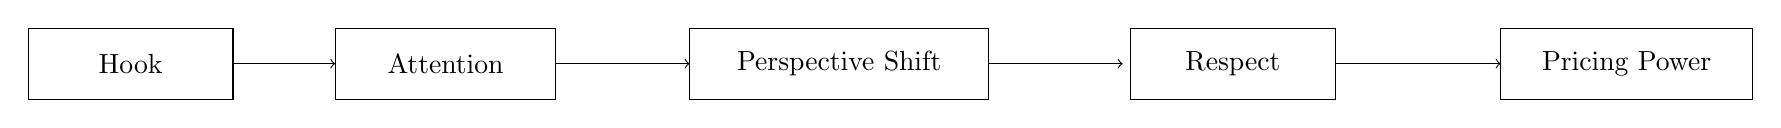
\begin{tikzpicture}
\node[draw, rectangle, minimum width=2.6cm, minimum height=0.9cm] (a) at (0,0) {Hook};
\node[draw, rectangle, minimum width=2.8cm, minimum height=0.9cm] (b) at (4,0) {Attention};
\node[draw, rectangle, minimum width=3.8cm, minimum height=0.9cm] (c) at (9,0) {Perspective Shift};
\node[draw, rectangle, minimum width=2.6cm, minimum height=0.9cm] (d) at (14,0) {Respect};
\node[draw, rectangle, minimum width=3.2cm, minimum height=0.9cm] (e) at (19,0) {Pricing Power};
\draw[->] (1.3,0) -- (2.6,0);
\draw[->] (5.4,0) -- (7.1,0);
\draw[->] (10.9,0) -- (12.6,0);
\draw[->] (15.3,0) -- (17.4,0);
\end{tikzpicture}
\caption{A transcript-derived branding funnel: the lecture's claim is that early attention and a perspective shift can be converted into respect and, eventually, into commercial leverage.}
\end{figure}

This first case therefore gives the chapter two linked ideas: pressure produces motion, and motion must quickly become legible to the market.

\section{Recurring Revenue, Systems, and Boring Businesses}

The tanning-salon owner changes the lecture's register. We move from personal brand and social media into repeatable business architecture. The surface business may look unglamorous, but the lecture uses it to make a stronger structural claim: the closer a business gets to repeatable, periodic payments, the more reliable the engine of wealth becomes.

The basic recurring-revenue notation is simple:
\begin{equation}
R_{\mathrm{rec}} = \sum_{t=1}^{T} r_t,
\end{equation}
where \(r_t\) denotes the cash inflow received at period \(t\). This is not the full economics of the business, but it is enough to preserve the lecture's distinction between a one-time payment and a payment stream.

The owner gives concrete scale markers:
\begin{equation}
N_{\mathrm{tan}} \approx 270,
\qquad
W_{\mathrm{tan}} > \$100\,\mathrm{M}.
\end{equation}
What the lecture wants us to hear is not merely that tanning salons made money, but that recurring billing plus systematized expansion can support very large wealth even in a business most people would never name first.

The second layer is the system itself. The owner cites the idea of acting as if one had \(500\) locations even when one had one. We may summarize that by the replication notation
\begin{equation}
S_1 \rightsquigarrow S_{500},
\end{equation}
where \(S_n\) denotes an operating system that remains valid when scaled from \(n=1\) to much larger \(n\).

\subsection{Question \& Answer}

\paragraph{Question.} Can we buy a real business even if we do not have much money?

\paragraph{Answer.} The lecture's answer is yes, but only within a specific market condition and a specific financing structure. The market condition is what the speaker calls the Silver Tsunami: many owners wish to retire, and there are not enough buyers. In symbols we may write
\begin{equation}
B_{\mathrm{sale}} > B_{\mathrm{buyers}}.
\end{equation}
Under that imbalance, owner financing becomes possible. In its simplest schematic form,
\begin{equation}
P = D + F_{\mathrm{seller}},
\end{equation}
where \(P\) is the purchase price, \(D\) is the buyer's down payment, and \(F_{\mathrm{seller}}\) is the seller-financed component.

The point is not that capital is irrelevant. The point is that the seller may accept part of the risk and become the lender when retirement pressure is high and buyer supply is low. That is why the lecture urges attention toward boring businesses rather than fashionable ones.

The short AI digression in this portion is awkward in pacing but still conceptually useful. The claim is not that AI abolishes work; it alters the labor requirement of a department. If \(50\) workers were once needed, the post-AI headcount may be smaller:
\begin{equation}
L_{\mathrm{after\ AI}} < 50.
\end{equation}
The transcript does not supply the replacement number, so we should keep the inequality qualitative.

\section{Industrial Real Estate and the Capital Question}

The real-estate developer introduces a different wealth grammar. Here scale is tied less to branding than to demand chains, timing, risk concentration, and access to investors. The lecture first motivates industrial real estate through a causal sequence:
\begin{equation}
\text{COVID e-commerce} \to \text{warehouses/distribution centers} \to \text{industrial demand}.
\end{equation}
This is the lecture's way of translating a broad social event into a specific asset class.

The numerical anchor in this section is the claim that a company begun in \(2019\) is now worth a little over \$4 billion:
\begin{equation}
V_{\mathrm{devco}} \gtrsim \$4\,\mathrm{B}.
\end{equation}
The lecture does not ask us to compute an internal rate of return; it asks us to understand the conjunction of experience, timing, and risk appetite.

\subsection{Question \& Answer}

\paragraph{Question.} Do we actually need a lot of money to get into real estate?

\paragraph{Answer.} The lecture's answer is no, if by that we mean cash already sitting in one's own pocket. But the answer is not that capital disappears. Rather, capital is assembled. The developer's claim is that one needs people who believe in the operator, share the vision, and expect to make money through that operator's judgment.

This is why the lecture treats investor trust almost as an asset:
\begin{equation}
\text{vision} + \text{credibility} \to \text{investor backing}.
\end{equation}
The same section ends with a second causal thesis, now about multi-residential real estate:
\begin{equation}
\text{lower liquidity} \to \text{shift from owning to renting}.
\end{equation}
That sentence matters because it shows the lecture's preferred style of argument. We do not begin with abstract theory. We begin with household balance-sheet pressure and infer the real-estate consequence.

\begin{figure}[h]
\centering
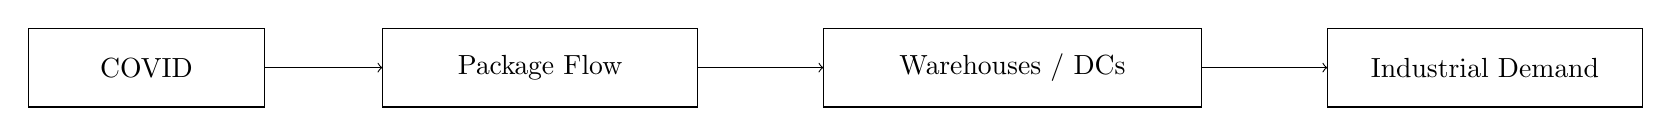
\begin{tikzpicture}
\node[draw, rectangle, minimum width=3cm, minimum height=1cm] (a) at (0,0) {COVID};
\node[draw, rectangle, minimum width=4cm, minimum height=1cm] (b) at (5,0) {Package Flow};
\node[draw, rectangle, minimum width=4.8cm, minimum height=1cm] (c) at (11,0) {Warehouses / DCs};
\node[draw, rectangle, minimum width=4cm, minimum height=1cm] (d) at (17,0) {Industrial Demand};
\draw[->] (1.5,0) -- (3,0);
\draw[->] (7,0) -- (8.6,0);
\draw[->] (13.4,0) -- (15,0);
\end{tikzpicture}
\caption{A transcript-derived demand chain for industrial real estate. The lecture explains the asset class through logistics rather than through abstract valuation alone.}
\end{figure}

\section{Ann Malum: Category Discovery, Word of Mouth, and the North Star}

Only now does the lecture return to its headline figure. That delay is important. By the time we arrive at Ann Malum's house, the lecture has already shown us several competing mechanisms of wealth. Ann's contribution is therefore not to repeat them but to fuse them.

The first step is category discovery. She describes success not as general cleverness, but as finding things before the public found them. This is why the Solidcore story starts with a workout that did not fit existing language: not exactly Pilates, not exactly strength training, not yet widely named. The lecture then shows how a category becomes legible through a memorable line, and how experience itself becomes marketing.

The key numerical statement is that Solidcore spent nothing on paid marketing during its first four years:
\begin{equation}
M_{\mathrm{paid}} = 0
\qquad
\text{for the first }4\text{ years.}
\end{equation}
The reason is the word-of-mouth loop:
\begin{equation}
\text{workout novelty} \to \text{soreness} \to \text{retelling} \to \text{new users}.
\end{equation}
The lecture does not present this as a formula, but it is exactly the kind of growth mechanism that the chapter ought to preserve. The product creates a sensation. The sensation produces a story. The story reduces the need for paid acquisition.

\subsection{Question \& Answer}

\paragraph{Question.} Why did Solidcore grow for years without paid marketing?

\paragraph{Answer.} Because the product itself generated retellable evidence. If a workout is sufficiently unfamiliar and sufficiently intense, it creates a conversation among customers. In that case marketing is not zero because nothing is happening; it is zero because the users are carrying the message.

The next structural element is the North Star. Ann says that from the beginning she knew the destination:
\begin{equation}
N_{\mathrm{target}} = 100.
\end{equation}
That target matters because it filters intermediate temptations. If one intends to reach \(100\) studios, then a sale offer or franchise possibility at \(10\) studios may be distraction rather than opportunity. The lecture's claim is not that all side paths are bad. It is that a sufficiently clear end state can keep the entrepreneur from confusing motion with progress.

This same section also answers a deeper question about entrepreneurship itself. Ann does not think everybody is built for it. Her language is that the real entrepreneur has something to prove, wants to win more than the rest, and chooses a game that matches a real personal edge. We may compress that closing rule as
\begin{equation}
q_{\mathrm{edge}} > q_{0.95},
\end{equation}
meaning that one should identify the thing one does better than about \(95\%\) of the population and attach that skill to a business that actually demands it. This is a heuristic, not a measurement protocol, but it is one of the lecture's strongest selection rules.

\section{After the Exit: Public Equities, Leverage, and the Compounding Game}

The final major movement of the lecture describes what changes once substantial wealth already exists. The discussion now becomes explicitly financial. Ann says that she is in wealth-preservation mode, though with meaningful risk tolerance. She gives a simple allocation statement:
\begin{equation}
w_{\mathrm{public}} \approx 0.50,
\qquad
H_{\mathrm{NVDA}} > \$10\,\mathrm{M}.
\end{equation}
She then gives the lecture's clearest distinction between rich and wealthy: once one has a large asset base, one can borrow against assets rather than liquidate them.

The specific borrowing structure is spoken in rough numbers:
\begin{equation}
L_{\mathrm{credit}} \approx \$50\,\mathrm{M},
\qquad
r_m \approx 5\%,
\qquad
t_{\mathrm{cg}} \approx 20\%.
\end{equation}
The transcript is garbled at one point, but the intended comparison is clear. Selling appreciated stock costs roughly \(20\%\) in capital gains tax; borrowing against the portfolio costs roughly \(5\%\).

\subsection{Question \& Answer}

\paragraph{Question.} Why would a wealthy person borrow against stock instead of selling it?

\paragraph{Answer.} Because the comparison is between the cost of borrowing and the cost of liquidation, not merely between borrowing and doing nothing. If the next opportunity is expected to return \(r_i\), and if
\begin{equation}
r_i > r_m,
\end{equation}
then the lecture's argument is that borrowing may dominate selling, especially when selling would crystallize a tax bill.

Ann's examples make the inequality concrete. She mentions deploying capital into startups, private companies, or loans yielding double digits:
\begin{equation}
r_i \in [12\%,15\%].
\end{equation}
Relative to a margin rate near \(5\%\), that is the spread the lecture wants us to see.

\subsection{A Worked Capital Example}

We can write the lecture's borrow-versus-sell logic in short steps.

\begin{enumerate}
\item Suppose we need capital for a new investment.
\item If we sell appreciated stock, we incur about \(t_{\mathrm{cg}} \approx 20\%\).
\item If instead we borrow, we pay about \(r_m \approx 5\%\) on the credit line.
\item If the next opportunity offers \(r_i \in [12\%,15\%]\), then \(r_i > r_m\).
\item On the lecture's logic, borrowing preserves the equity base, avoids realizing gains, and still allows capital deployment.
\end{enumerate}

The lecture then widens again and moves from leverage to compounding. Ann gives portfolio values at two moments in time:
\begin{equation}
W_{\mathrm{low}} \approx \$39\,\mathrm{M},
\qquad
W_{\mathrm{later}} \approx \$64\,\mathrm{M},
\qquad
\Delta W_{\mathrm{day}} \approx \$1.2\,\mathrm{M}.
\end{equation}
The conceptual law behind these statements is not mysterious:
\begin{equation}
W_{t+1} = (1+r_t)W_t.
\end{equation}
This is the chapter's cleanest expression of the lecture's phrase that money wants to make money and compound. The formula is standard, but here it should be read as a faithful compression of the spoken financial worldview rather than as a separate mathematical insertion.

Finally, the lecture contrasts this with the passivity of idle bank balances:
\begin{equation}
r_{\mathrm{bank}} < 0.5\%.
\end{equation}
That number is not offered as universal market data; it is the lecture's shorthand for the complaint that a savings account yields too little while the bank itself deploys the capital elsewhere.

\section{Summary}

The lecture begins with wealth as spectacle and ends with wealth as structure. Along the way we are shown several distinct machines: pressure converted into motion, attention converted into pricing power, recurring payments converted into business stability, retiring owners converted into acquisition opportunities, logistics converted into industrial demand, category confusion converted into word of mouth, and finally an asset base converted into leverage and compounding.

If we compress the entire chapter to one line, it is this: the lecture treats wealth as the result of building value once, systematizing it, and then learning the capital game well enough that the accumulated base can be preserved, borrowed against, and compounded. The glamour remains visible at the surface, but the chapter's work is to keep tracing it back to the underlying equations, however simple, that actually govern the story.